\documentclass[10pt,twocolumn,letterpaper]{article}

\usepackage{cvpr}
\usepackage{times}
\usepackage{epsfig}
\usepackage{amsmath}
\usepackage{amssymb}

\usepackage{booktabs} % for much better looking tables
\usepackage{array} % for better arrays (eg matrices) in maths
\usepackage{paralist} % very flexible & customisable lists (eg. enumerate/itemize, etc.)
\usepackage{verbatim} % adds environment for commenting out blocks of text & for better verbatim
\usepackage{subfigure} % make it possible to include more than one captioned figure/table in a single float
\usepackage{graphicx}
% Include other packages here, before hyperref.

% If you comment hyperref and then uncomment it, you should delete
% egpaper.aux before re-running latex.  (Or just hit 'q' on the first latex
% run, let it finish, and you should be clear).
%\usepackage[pagebackref=true,breaklinks=true,letterpaper=true,colorlinks,bookmarks=false]{hyperref}

\cvprfinalcopy % *** Uncomment this line for the final submission

\def\cvprPaperID{****} % *** Enter the CVPR Paper ID here
\def\httilde{\mbox{\tt\raisebox{-.5ex}{\symbol{126}}}}

% Pages are numbered in submission mode, and unnumbered in camera-ready
\ifcvprfinal\pagestyle{empty}\fi
\begin{document}

%%%%%%%%% TITLE
\title{
Project in CSE 250B\\
Assignment 2: Logistic Regression with Regularization}

\author{Andreas Landstad, Spencer Bliven, Jonas Hoelzler\\
Computer Science Department\\
University of California, San Diego\\
{\tt\small landstad.andreas@gmail.com, sbliven@ucsd.edu, jonas@hoelzler.de}
}% For a paper whose authors are all at the same institution,
% omit the following lines up until the closing ``}''.
% Additional authors and addresses can be added with ``\and'',
% just like the second author.
% To save space, use either the email address or home page, not both
%\and
%Second Author\\
%Institution2\\
%First line of institution2 address\\
%{\tt\small secondauthor@i2.org}
\maketitle
\thispagestyle{empty}

%%%%%%%%% ABSTRACT
\begin{abstract}
This project evaluates an email analytics dataset describing two email campaigns and a control group using machine learning methods. The datasets is analyzed using logistic regression with stochastic gradient descent as optimization method and a real-valued nonlinear regression training method.
The results show, that future mails should be sent to ???
\end{abstract}

%%%%%%%%% BODY TEXT
\section{Description of the Dataset}
Kevin Hillstrom, a well-known data mining consulatant has published an email analytics dataset with 64,000 records each describing a customer \cite{hillstrom08}. One third of these customers were randomly chosen to receive an email referred to as the Men's email, a
second random third received a different email (the Women's email) and the remaining customers served as a control, receiving neither email.
The dataset is almost perfectly equally divided between the two mailings (�Men's� and �Women's�) and an untreated control group (see Table \ref{dataoverview}).


\begin{figure}[htb]
	\centering

 \begin{tabular}{|l|l|l|l|l|}
  \hline
   Mailing & Men    & Women  & None   & Total   \\
   \hline 
   Count & 21,307 & 21,387 & 21,306 & 64,000 \\
   \%       & 33.29\% & 33.42\% & 33.29\% & 100.00\% \\
   
  \hline
 \end{tabular}

\caption{Encoding}
 \label{dataoverview}
\end{figure}

\section{Preprocessing of the Dataset}
The data is given as a comma separated file. To apply the logistic and linear regressions, the data has to be preprocessed. For the learning algorithm, the rows of the dataset are encoded in 29-dimensional $x$-vectors.

First, the recency entry shows the number of months since the last purchase from one to twelve months. In this project it is encoded as a bit-vector of eleven bits (bit 1 to 11), where the $i$th bit is $1$ for a recency of $i$ months and $0$ otherwise. The $12$th bit is left out, since it only represents redundant information.
The history segmentation is a categorization of the customers in 7 categories, using how many dollars were spent in the last year.
It is encoded again as bit-vector 12 to 17, while one bit is again left out due to redundancy.
Entry 18 shows the real value of actual dollars spent in the past year. Entry 19 and 20 are true, if the customer purchased men's respectively women's merchandise in the past year. Bit 21 and 22 categorize the customer in its zip code area. Bit 21 is $1$, if he is from a rural area, bit 22 is $1$, if he is from a urban area. The bit for the suburban area is again left out.
Bit 23 is the indicator, if the customer is a new customer mentioned the last twelve months.
The channel describes the channel the customer purchased  from  in the past year. Bit 24 is $1$ for the phone, bit 25 is $1$ for the web. The bits are not mutually exclusive. 

Because the learning rate is the same for every parameter, it is useful to scale the features $x_j$ so that their magnitudes are similar for all $j$. The features are normalized having mean zero and variance $1$ \cite{elkan11}.

 
Hillstrom provides three outcome (dependent) variables indicating whether people visited the site during a two-week outcome period, whether they
purchased at the site (�conversion�) during that period, and how much customers spent during the outcome period (zero, for those who
didn't).





\begin{figure*}[tb]
	\centering
 	\begin{tabular}{|c|c|c|c|c|c|c|c|c|c|c|c|c|c|c|c|c|c|}
  	\hline
  	 1&2&3&4&5&6&7&8&9&10&11&12&13&14&15&16&17\\ 
  	 \hline
  	 \multicolumn{11}{|c|}{Recency}&\multicolumn{6}{|c|}{History segment}\\
  	 \hline
		1&2&3&4&5&6&7&8&9&10&11&\$0-\$100&\$100-\$200&\$200-\$350&\$350-\$500&\$500-\$750&\$750-\$1000\\ 
  	\hline
 		\end{tabular}
 		


 		\begin{tabular}{|c|c|c|c|c|c|c|c|c|c|c|}
  	\hline
  	 18&19&20&21&22&23&24&25&26&27&28\\ 
  	 \hline
  	 History&Mens&Womens&\multicolumn{2}{|c|}{Zip-Code}&Newbie&\multicolumn{2}{|c|}{Channel}&Visit&Conversion&Spent\\
  	 \hline
		H&M&W&U&R&N&P&W&V&C&S\\ 
  	\hline
 		\end{tabular}
\caption{Encoding}
    \label{encoding}
\end{figure*}


\subsection{Model of Computation}
As one can see in Table \ref{dataoverview}, the customers are divided into three groups. For each of these groups the same computational model can be applied. These three submodels are part of the overall model

\[E[spend|x,treatment] = E[spend|purchase,x,treatment] \]
\[ *\ p(purchase|visit,x,treatment)\ *\ p(visit|x,treatment) \]
This eqauation is applied to all three groups, called $treatment$ in the equation with the possible values $women's\ clothing$, $men's\ clothing$ and $no\ email$. $x$ is the vector of attribute values described in the section above. $visit$ and $purchase$ are binary random variables that have a certain probability of being true of false for each customer. $spend$ is a real-value random variable for each customer.

Goal of this equation is to find out, how much money the customer spent, given a particular treatment. The probability $p(visit|x,\ treatment)$ is the probability, that a customer visits. $p(purchase|visit,\ x,\ treatment)$ is the probablity that the customer purchases. $E[spend|purchase,\ x,\ treatment]$ is the expected real-valued outcome for a customer. These three terms have to be multiplied, since a customer, who spends money has also to visit the store and to purchase anything.



\section{Logistic and Linear Regression}
The three terms of the equation above can be calculated by logistic regression and linear regression.
This can be applied to the second and third term. The first term can be calculated using linear regression.

\subsection{Logistic Regression}

\renewcommand{\b}{\boldsymbol{\beta}}

Logistic regression is
 %a special case of conditional likelihood and
 a common model for binary classification \cite{bishop06}. Given an example $\mathbf{x} \in\mathbb{R}^d$, the probability of a label $y\in\{0,1\}$ is given by the logistic sigmoid function
\[p(Y=1\ |\ X=\mathbf{x};\ \b) = \frac{1}{1+\exp(-\b\cdot \mathbf{x})} \]
where $\b$ is a $d$-dimensional vector. We assume $x_0=1$ such that $\b_0$ acts as an intercept.
Given a set of parameters $\b$, the logistic function can be used for classification:
\[ \hat{y} = \operatorname*{arg\,max}_y\,p(Y=y\ |\ X=\mathbf{x};\ \b) \]

To learn useful parameters $\b$ we utilize a training set $(X,Y) = \left\{ (\mathbf{x}_i,y_i)\ |\ i=1\dots N \right\}$. The optimal $\b^*$ is chosen such that it maximizes the regularized log conditional likelihood over the training set
\begin{align*}
\b^* &= \operatorname*{arg\,max}_{\b}\,LCL(\b;\ Y|X) - \alpha \, \parallel \b \parallel^2 \\
&= \operatorname*{arg\,max}_{\b}\,\sum_{i=1}^{N} \log p(y_i\ |\ \mathbf{x}_i;\ \b) - \alpha \, \parallel \b \parallel^2 .
\end{align*}
The optimal $\b^*$ is found numerically using stochastic gradient descent (SGD). An initial $\b_0 = \mathbf{0}$ is chosen. For each example in the training set, $\b$ is updated according to the rule
\begin{align*}
\b_{t+1} &= \b_{t} + \lambda \, \nabla  \left( LCL_i(\b;\ Y|X) - \alpha \, \parallel  \b \parallel^2 \right) \\
&= \b_{t} + \lambda \,\left( \left(y_i-p_i\right)\, \mathbf{x}-2\alpha \b \right)
\end{align*}

\subsection{Linear Regression}
Missing


\section{Complexity Analysis}

Each update step of SGD requires computing the gradient with respect to $\b$ of regularized LCL for the current example. For $d$ dimensions this takes time $O(d)$. Thus each epoch of SGD 

\section{Implementation}


\section{Evaluation}


\begin{figure*}[htbp]
  \centering
  \begin{minipage}{5.5 cm}
    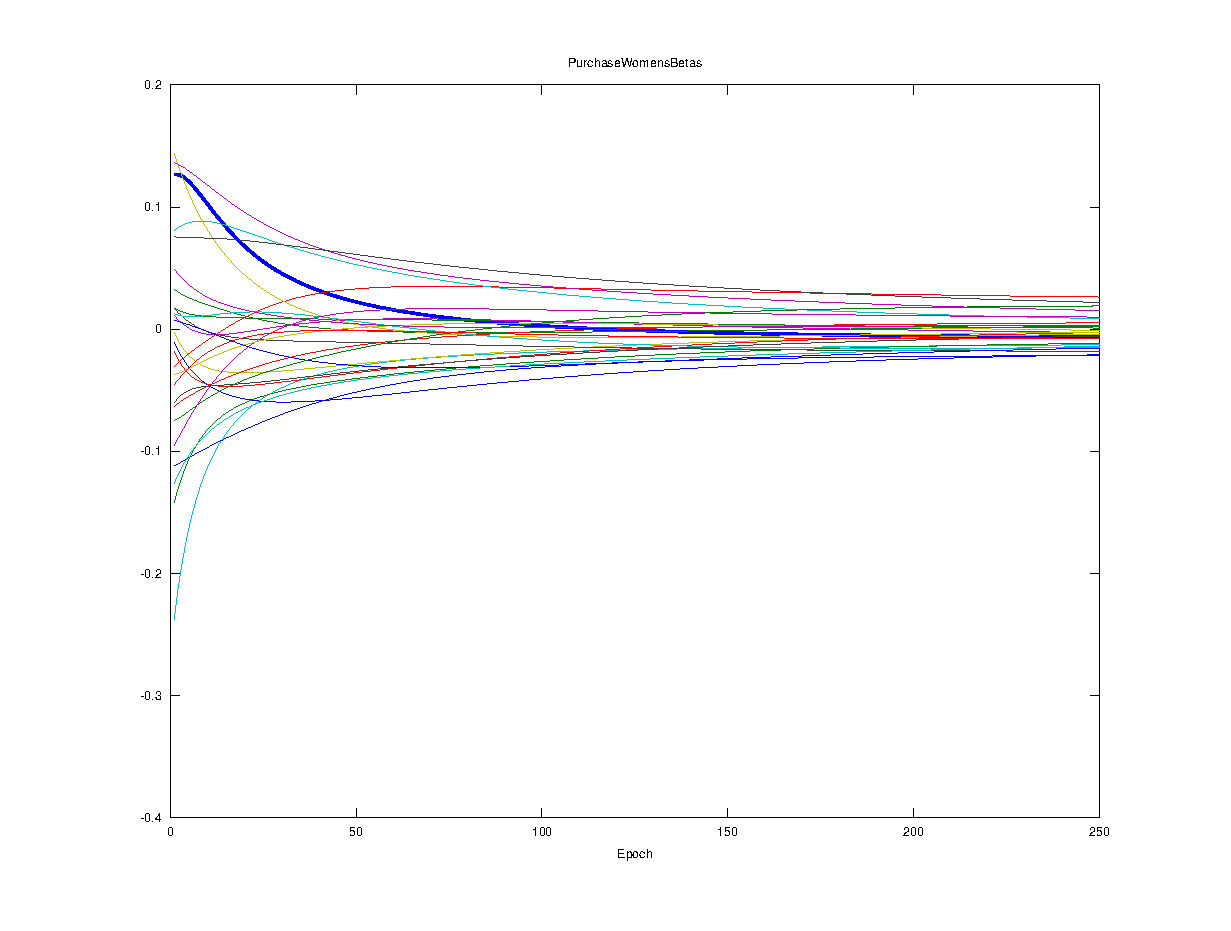
\includegraphics[width=5.5cm]{PurchaseWomensBetas}  
  \end{minipage}
  \begin{minipage}{5.5 cm}
    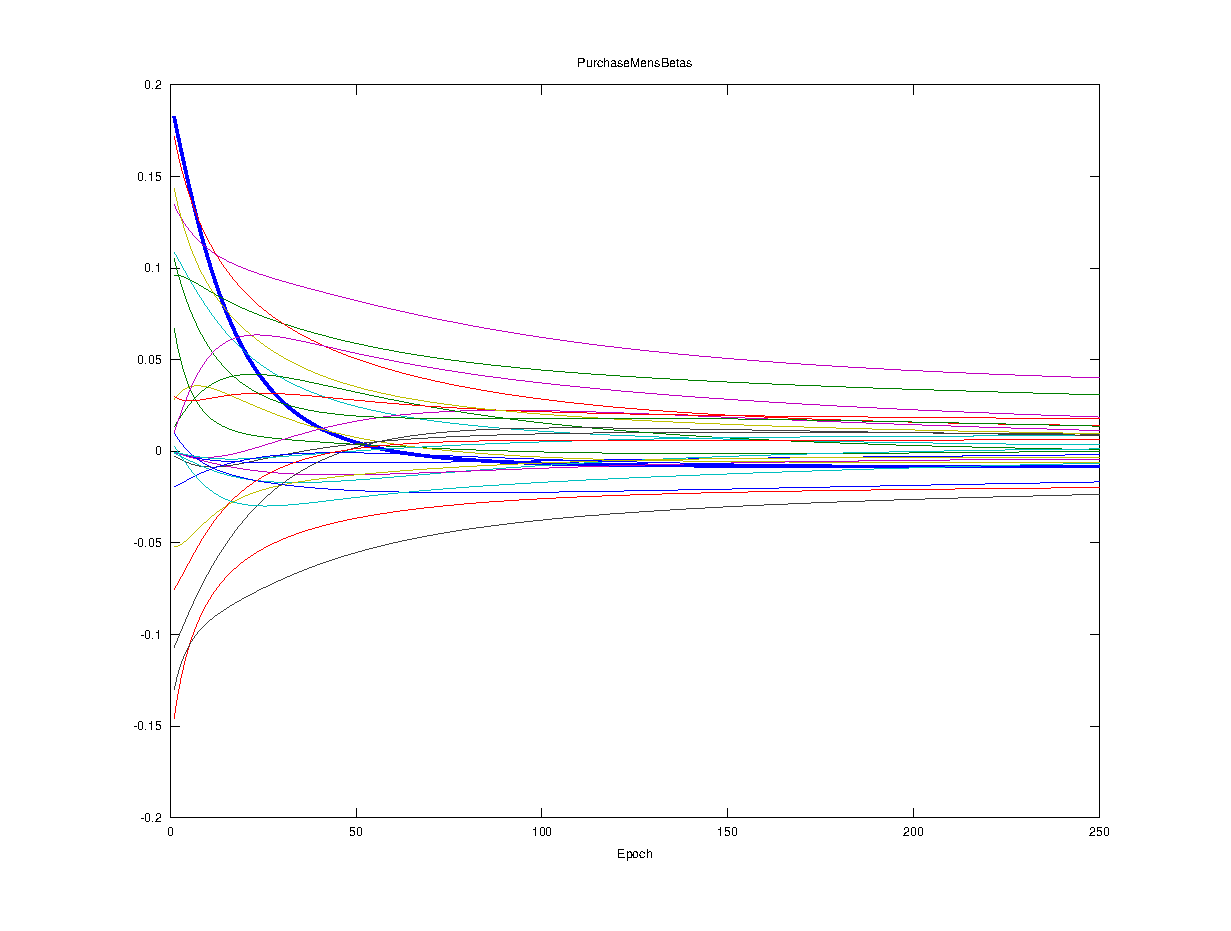
\includegraphics[width=5.5cm]{PurchaseMensBetas}  
  \end{minipage}
  \begin{minipage}{5.5 cm}
    \includegraphics[width=5.5cm]{PurchaseNoEmailBetas}  
  \end{minipage}
  \caption{Purhase Betas Conversion}
  \label{Labelname}
\end{figure*}



%------------------------------------------------------------------------

\section{Conclusions}


\nocite{hillstrom08, bishop06,bottou11,elkan11}

{\small
\bibliographystyle{ieee}
\bibliography{egbib}
}

\end{document}
